\documentclass{article}
\usepackage[utf8]{inputenc}
\usepackage{titling}
\usepackage{graphicx}
\usepackage{xcolor}
\usepackage[colorlinks=true,linkcolor=darkgray, urlcolor =gray]{hyperref}
\usepackage[spanish]{babel}
\DeclareUnicodeCharacter{301}{~}
\usepackage{url}
\DeclareUnicodeCharacter{202F}{\,}


\title{Ejercicios Optativos 2}
\author{Cristina Díaz García}
\date{Diciembre 2018}

\renewcommand\maketitlehooka{\null\mbox{}\vfill}
\renewcommand\maketitlehookd{\vfill\null}


\begin{document}

\addcontentsline{toc}{section}{Índice general}

\begin{titlingpage}
\maketitle

\begin{center}
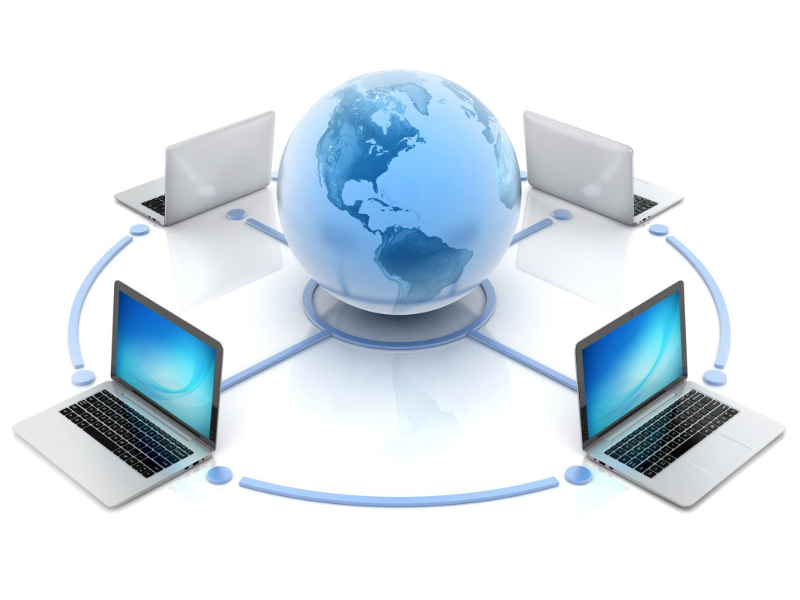
\includegraphics[scale=0.4]{images/comunicaciones.png} 
\end{center}

\end{titlingpage}

\newpage

\tableofcontents

\newpage

\section{I. Desarrollo de servicios no estándar}


\subsection{Ejercicio 2}.

2. Implementar el mismo servicio de “eco” que en el ejercicio anterior pero esta vez sobre
TCP. Deberán tenerse en cuenta los siguientes requisitos de implementación:
\begin{itemize}
\item Usar la interfaz \textit{Executor} para implementar el servidor concurrente.
\item Opcionalmente implementar la otra opción de grupo de hebras y comparar ambas
implementaciones
\item El cliente le notificará al servidor el final del servicio mediante el cierre del \textit{socket}.
\end{itemize}

En este ejercicio se han implementado tres clases:

\begin{itemize}
\item \textbf{TCPCliente:} Es el cliente, al que se le pasan como argumentos al ejecutarlo, primero la dirección IP a la que conectarse, y segundo, el puerto. Si el servidor no estuviera disponible, el cliente se cierra automáticamente. En caso de que se realizara la conexión, envía y recibe los mensajes hasta que se envía un punto, en cuyo caso, el servidor cierra la conexión y el cliente se cierra.
\begin{center}
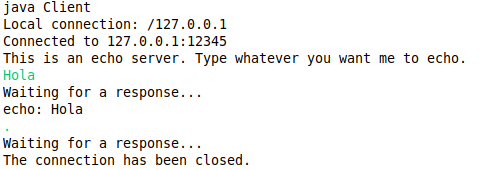
\includegraphics[scale=0.4]{images/TCPClient.png}
\end{center}
\item \textbf{TCPServer:} Es el servidor, al que se le pasa como argumento el puerto por el que escuchar. Cada vez que un cliente se intenta conectar, se crea una instancia de EchoProtocol, que es el que ``gestiona" la conexión, es decir, es el que hace la función de eco.
\begin{center}
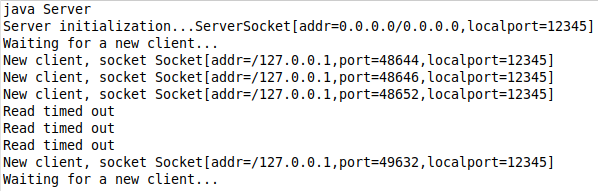
\includegraphics[scale=0.4]{images/TCPServer.png}
\end{center}
\item \textbf{EchoProtocol:} Recibe los mensajes del cliente y se los reenvía, siempre que el mensaje no fuera un punto, en cuyo caso cerraría la conexión.
\end{itemize}

Las ventajas de la implementación con TPC es la fiabilidad de la conexión. En esta implementación, uno de los problemas que tenemos es que estamos asumiendo que los argumentos se van a introducir tanto en el orden correcto como siendo los necesarios, es decir, no vamos a meter una IP incorrecta, ni vamos a introducir una palabra en vez de la IP correspondiente.

\subsection{Ejercicio 3}

3. A partir del servicio de “eco” dado en clase realizar las siguientes modificaciones para
probar las diferentes opciones de sockets sobre TCP:
\begin{itemize}
\item En el servidor, limitar el tiempo de espera de una nueva conexión dando por finalizado
el servidor tras dicho tiempo (ej: varios minutos). Nota: probar a arrancar el servidor
justo después de su finalización, antes de implementar la característica que se propone
a continuación, ¿qué ocurre?
\item En el servidor establecer la opción de reutilización del puerto para facilitar el arranque
del servidor tras su finalización por el temporizador
\item En el servidor, limitar el tiempo total del servicio de “eco” (ej: un minuto)
\item Cambiar en el cliente el tamaño del buffer de escritura a 512 bytes y comprobar si se
ha cambiado visualizando el valor anterior y el nuevo.
\item Deshabilitar el algoritmo de Nagle, que es especialmente recomendado si se va a
realizar el eco a nivel de caracteres o mensajes muy pequeños.
\end{itemize}

\section{Quiz 2}

La señal más baja es aquella de la que más se pierde la señal, y mientras más mayor el valor absoluto del RSSI negativo, mayor es la pérdida de señal.

\begin{center}
\includegraphics[scale=0.3]{WLAN/signal.png} 
\end{center}

La gráfica de la evolución temporal es la siguiente:

\begin{center}
\includegraphics[scale=0.3]{WLAN/chart.png} 
\end{center}

Siempre está en el canal 11 excepto en el paquete 322, que está en el 6, como podemos comprobar:

\begin{center}
\includegraphics[scale=0.3]{WLAN/channel11.png} 
\end{center}

\begin{center}
\includegraphics[scale=0.3]{WLAN/channel6.png} 
\end{center}

\section{Quiz 3}

En este ejercicio el problema es que ciertos paquetes tienen errores en con el checksum o el payload.

\begin{center}
\includegraphics[scale=0.3]{WLAN/malformed.png} 
\end{center}

El tráfico es todo 802.11:

\begin{center}
\includegraphics[scale=0.3]{WLAN/802_11}
\end{center}
\begin{center}
\includegraphics[scale=0.3]{WLAN/not802_11}
\end{center}

Todo el tráfico coloreado de blanco es de tipo broadcast (802.11) y el negro de tipo error en el checksum.

\begin{center}
\includegraphics[scale=0.6]{WLAN/documentacion.png} 
\end{center}

\begin{thebibliography}{9}

\bibitem{Colores} \textit{Coloring rules}, \url{http://manualwireshark.blogspot.com/}.

\end{thebibliography}

\end{document}